\section{Observational Design Study}
\label{sec:abs_study}
In this observational design study, we wanted to observe how groups of people with varying levels of expertise in art would work together on a drawing task, and see how collaboration would be affected by usage of abstraction strategies. While the experts we observed used abstract composition sketches to create the ``undersketch'' of their eventual drawing, we anticipated that most of our participants would not know how to do this. 

\subsection{Method}

\subsubsection{Participants}
Six groups of two to four people ($n=$ 19, 11 female, average age $=$ 28 years) participated in a collaborative drawing task. Participants were recruited from a technology company and local art school through an email advertisement and signed up for scheduled time slots. Though group members were not required to know each other, at least two people from each group had an existing working relationship. The average self-reported drawing experience level was 1.95 ($SD=$ 0.78) out of 4, with 1 being no experience and 4 being expert level. We randomly assigned groups to two conditions: three to \textit{abstraction} and three to \textit{freeform}. Each condition comprised one group of size two, one group of three, and one group of four to explore how communication potentially changes as function of group size. While most groups were co-located, one group in each condition consisted of distributed participants using an online shared canvas (Google Jamboard) and video conferencing (BlueJeans). Observing these distributed groups gave insight on the impact of abstraction on co-located versus remote collaboration. Participants received a \$25 USD gift card for their time. All sessions were video and audio recorded with the experimenter taking note of critical moments during each session.  

\subsubsection{Procedure}
For \textit{abstraction} groups, we first presented a short tutorial of how to use abstraction blocks (Figure \ref{fig:blocks}). Our tutorial explained that participants could use the blocks to represent where a sketch element would be in a drawing. They were free to use text, sketches, or the blocks as they pleased. Groups each made a collective drawing in response to the prompt, ``A scene with a time-traveling tourist.'' We chose a fictional storytelling prompt and drawing task because it does not require any domain knowledge and enables collaborative ideation and interaction \cite{Davis2017}. The task was 20 minutes long and broken into three segments to control for time spent in each part of the process across conditions: five minutes for brainstorming, five minutes for planning and drafting, and ten minutes for drawing. Groups could use paper, pens, pencils, and colored pencils throughout the task. We asked each group to deliver their drawing on one sheet of paper by the end of the study session.

During brainstorming, participants discussed ideas without worrying about drawing yet. Before the planning phase, we gave a short explanation of basic composition concepts and instructed groups to focus on drawing composition during planning. \textit{Abstraction} groups were given standard size and small sticky notes to use and presented with the blocking strategy at this time. Google Jamboard's sticky note feature and pen tools simulated using physical sticky notes and regular analog sketching in the remote sessions. \textit{Freeform} groups were able to plan their drawing in any manner. Following planning, groups collaboratively worked on their drawing for the remainder of the task. Directly after the drawing task, the experimenter replayed recorded critical moments on a computer screen for groups (and through the sharescreen feature for digital groups), asked them to reflect on these clips, and reviewed any additional moments mentioned during the discussion. 

\subsection{Results}
To find emergent themes of how groups interacted with drawing artifacts and each other, we noted interesting behaviors and critical moments in each of the sessions, looking for commonalities across groups and between conditions. We found that groups that used abstraction blocks engaged in more conceptual discussion and worked together in a more flexible manner.

\subsubsection{Abstraction Enabled Integrated Collaboration} 
Compared to freeform sketching, abstraction blocks seemed to help groups form a strong shared understanding of each others' ideas. To represent drawing elements, \textit{abstraction} groups placed sticky notes on their draft paper to create a blueprint of their composition. For example, Group 2 (\textit{abstraction}) put three sticky notes together to represent a focal point (a train) of their drawing while using the smaller sticky notes to represent smaller elements (individual people). These sticky notes were labeled with a brief written description or a small sketch showing what the block was supposed to represent.

\begin{figure*}
\centering
  \vspace{-0.2in}
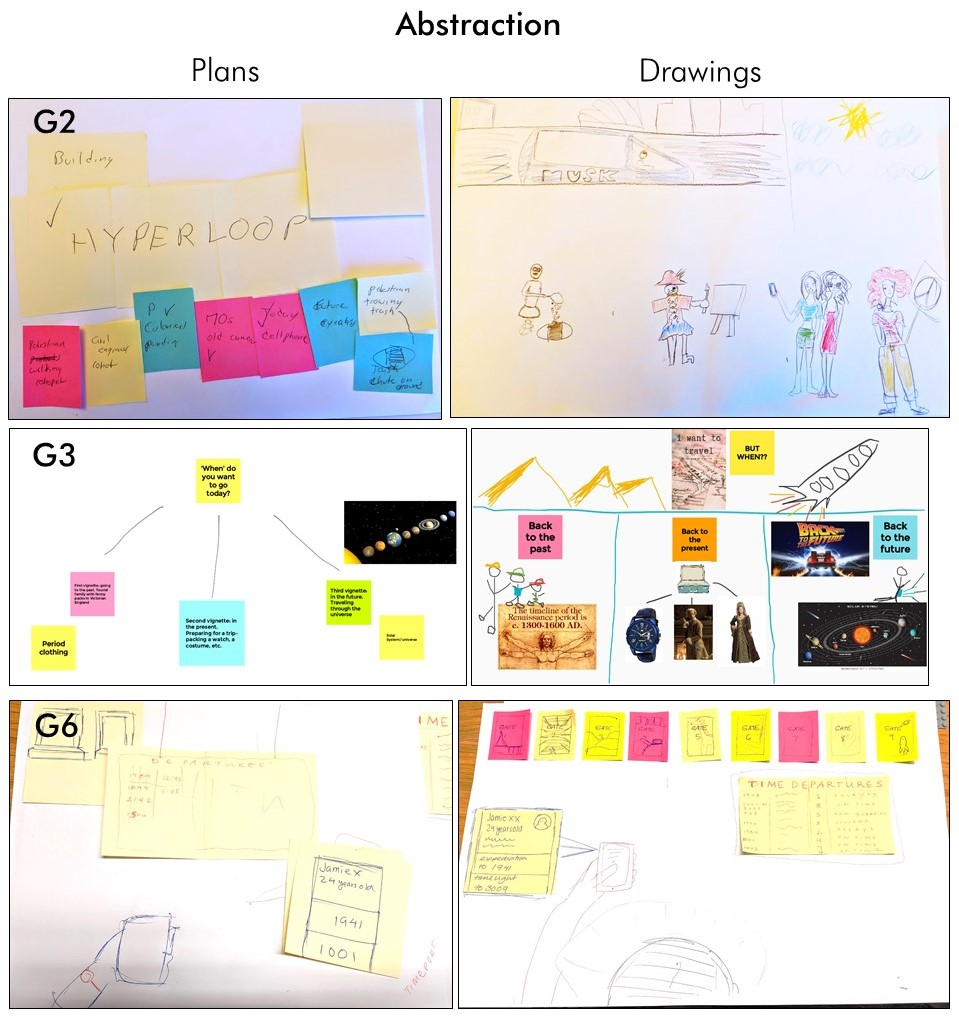
\includegraphics[width=\textwidth]{abstraction/figures/abs.jpg}
% 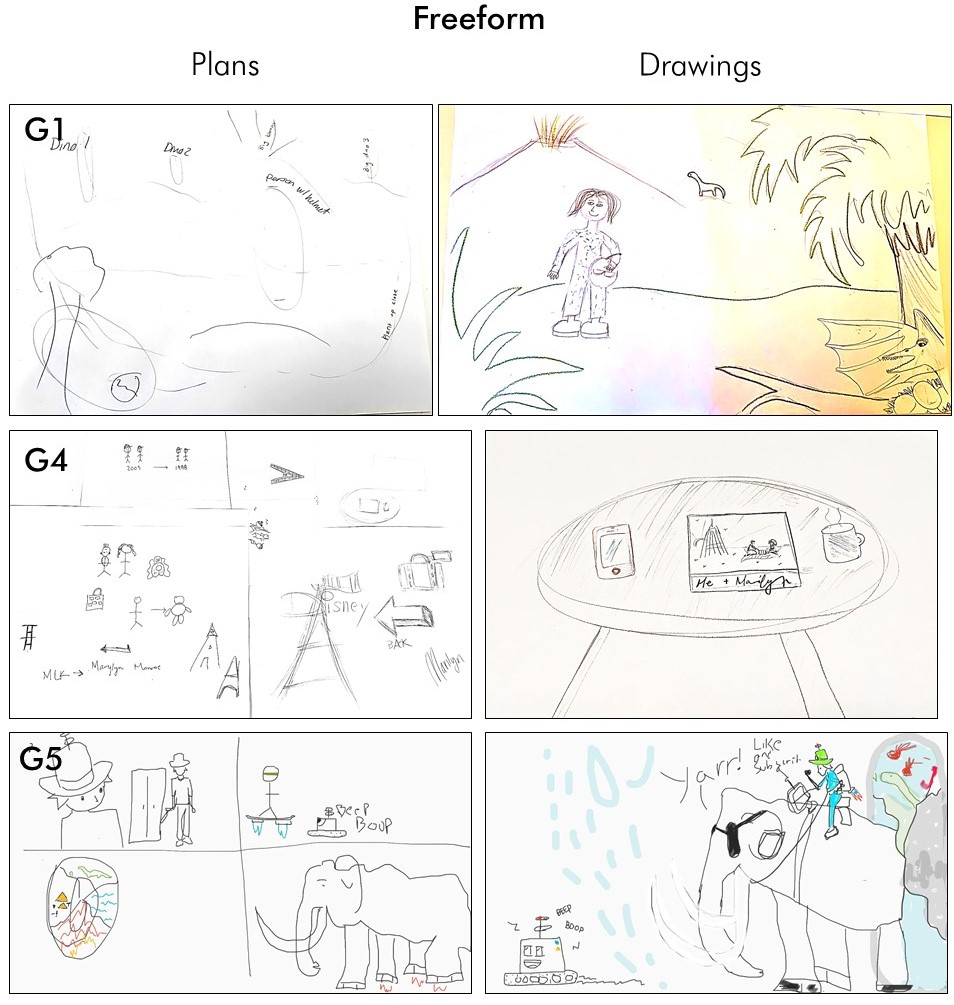
\includegraphics[width=\textwidth]{abstraction/figures/freeform.jpg}
\vspace{-0.3in}
  \caption{\textit{Abstraction} groups developed composition plans from the abstract blocks that formed the basis of their final drawings.}
  ~\label{fig:abs_drawings}
  \vspace{-0.2in}
\end{figure*}

\begin{figure*}
\centering
  \vspace{-0.2in}
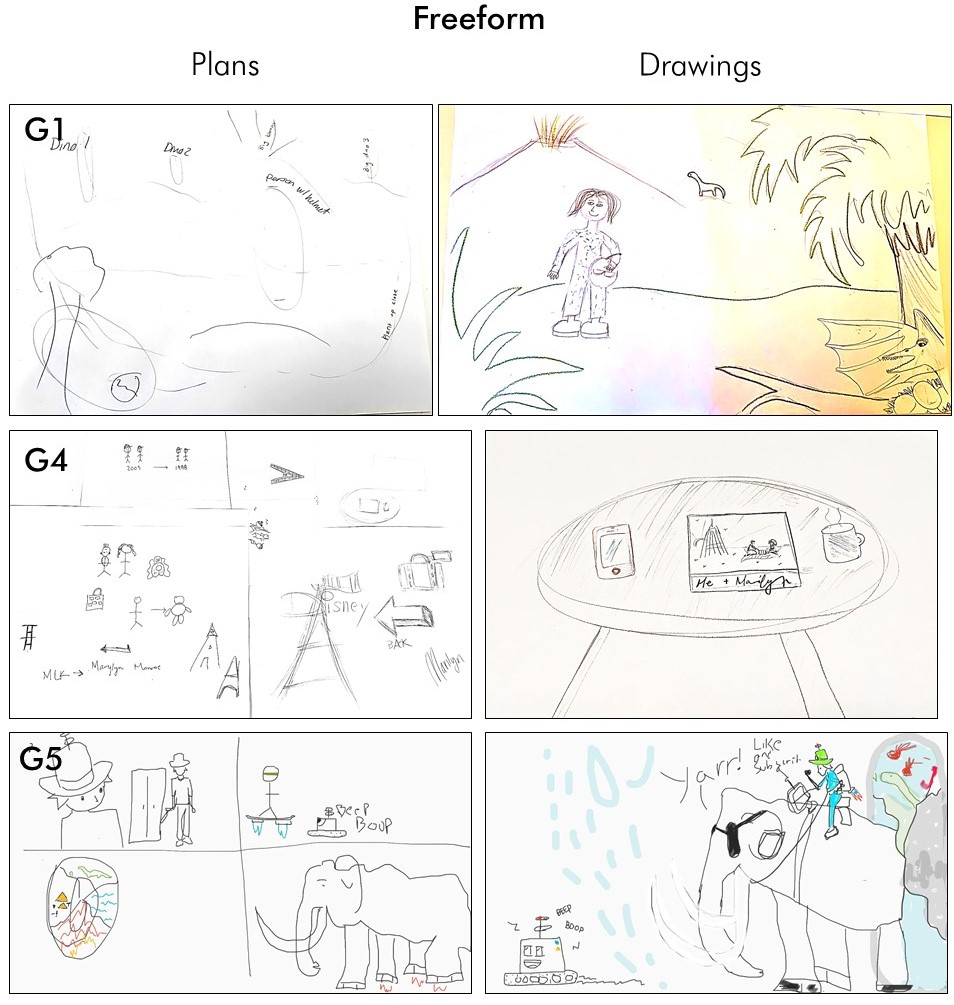
\includegraphics[width=\textwidth]{abstraction/figures/freeform.jpg}
\vspace{-0.3in}
  \caption{\textit{Freeform} groups tended to sketch individual details before deciding on a final composition.}
  ~\label{fig:freeform_drawings}
  \vspace{-0.2in}
\end{figure*}

Similar to the thumbnail sketches created by the experts we observed, abstraction blocks helped anchor discussion by providing shared representations of what members of the group were thinking about: \textit{``I think once someone gave us a visual view of what [they were] thinking, I feel like we all were like ‘Yeah! Perfect'.''} (P5, \textit{abstraction}). P6 (\textit{abstraction}) similarly said in the post-interview that \textit{``everyone has different ways of placing things on paper so once we laid out that this goes here, I think it was helpful for all of us to just visualize the layout of all the things we were talking about.''}

In contrast, Group 1 was the only \textit{freeform} group to make a lightly sketched blueprint of their drawing due to one participant's prior domain knowledge in photography and compositions. 

In other \textit{freeform} groups, participants sketched their own individual drawing elements on separate sheets of paper or divided up their shared drawing sheet into areas ``owned'' by each member of the group (Figure \ref{fig:freeform_drawings}). For example, Group 4 members each sketched their own version of the Eiffel Tower on their scratch paper. 
For \textit{freeform} groups, planning seemed to be oriented around making decisions about specific details of the drawing rather than explore options for the drawing's overall composition.

These differences in how groups approached planning their drawing also affected how they allotted drawing work among individuals. \textit{Abstraction} groups tended to use the blocks they had created as a way to define who should draw what. For example, Group 2 (\textit{abstraction}) assigned each person to draw one of the block elements on their composition plan. They physically checked off the blocks on their plan as they were drawing to mark which ones they completed:

\begin{quote}
    P3: \textit{``I can take `colonial' [people].''}\\ 
    P5: \textit{``We'll take the `today' people on this side.''}\\
    --- Group 2 (\textit{abstraction})
\end{quote}

\textit{Freeform} groups focused instead on smaller, individual elements and focused on the details of these elements. For example, Group 1 (\textit{freeform}) split up their work by individual characters: \textit{``So do you want to start drafting the person and play around with outfits, and I'll do the dinosaurs?''} (P1, \textit{freeform}). However, because \textit{freeform} participants had individually planned portions of the drawing separately from others in their group, they encountered conflicts in their understanding of the drawing's composition as sketching progressed.

One \textit{freeform} participant in Group 5 asked another group member to redraw and switch the orientation of another element during drawing: \textit{``Can you draw the portal on the right because I drew the mammoth from right to left, and this will be very complicated for me to draw it from left to right.''} (P16 \textit{freeform}). There was also sometimes confusion about what each person should work on during drawing. In the post-interview, P13 (\textit{freeform}) said, \textit{``I didn't quite know what I was doing, everyone seem to have their own parts...and I was like 'what should I do?'''}. P14 (\textit{freeform}) also mentioned that he wished his group had done more concrete outlining beforehand so \textit{``people can work more independently instead of having to wait for another part to be done.''} 

\subsubsection{Abstraction Groups Focused on High-Level Decisions}
Groups that used abstract blocks seemed to discuss higher-level concepts like general theme and layouts throughout the drawing process. For example, when talking about how to depict a person looking at a time travel app on his phone, Group 6 (\textit{abstraction}) included light sketches on their blocks (Figure \ref{fig:abs_drawings}) to capture and discuss concepts like point of view, background focus, and scale during planning:

\begin{quote}
    P19: \textit{``Maybe we're still in his point of view, like he's looking at his phone.''}\\
    P17: \textit{``The scale can be small because we probably don't want to get too detailed, but the idea is just to convey that it's a travel app.''}\\
    P18: \textit{``And maybe we can have a thing where it's like zoomed in to show this is what he's holding.''}\\
    --- Group 6 (\textit{abstraction})
\end{quote}

Group 3 (\textit{abstraction}), the digital group, spent their planning time setting high-level goals for their drawing. They made blocks with questions for what they wanted to achieve in their drawing rather than making individual sketches: \textit{``Do you wanna have the main question on the top, and then like three vignettes below?''} (P8, \textit{abstraction})

\begin{figure}[b!]
\centering
  \vspace{-0.25in}
  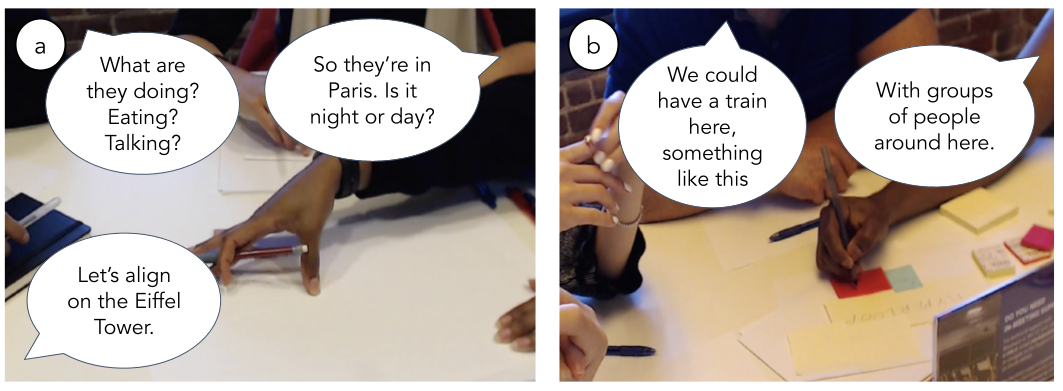
\includegraphics[width=.9\columnwidth]{abstraction/figures/planning.png}
  \caption{(a) \textit{Freeform} groups discussed details early without making concrete sketches until their final drawing. (b) \textit{Abstraction} groups instead used abstract blocks to concretely discuss and sketch a drawing composition.}~\label{fig:tangible}
  \vspace{-0.2in}
\end{figure}

\textit{Freeform} groups instead had a tendency to discuss lower-level details during planning, corroborating findings from prior work \cite{jansson1991design, Little2010, Yu2016}. In Group 5 (\textit{freeform}), participants discussed incremental details for how specific elements should look. For example, when discussing how to show a time traveller coming out of a time travel portal:

\begin{quote}
    P15: \textit{``We could have different futures in the portal, like maybe one where the world is flooded.''}\\
    P14: \textit{``Looks like [P15] has gone in pretty hard on [drawing] the portal...so [P13] should draw the traveler.''}\\
    P15: \textit{``And then [P14] will add lasers to it.''}\\
    P14: \textit{``Yeah like laser accessories.''}\\
    --- Group 5 (\textit{freeform})
\end{quote}

Discussions would often chain together incrementally, adding more details to existing ideas rather than offering new directions to explore. For example, Group 4 (\textit{freeform}) similarly attended to details and discussed the specifics of what their subjects would be doing in their drawing despite being in the planning stage of the study session:

\begin{quote}
    P12: \textit{``What are they doing? Talking?''}\\
    P9: \textit{``Eating?''}\\
    P11: \textit{``Yeah, wine. Eating.''}\\
    P12: \textit{``Coffee?''}\\
    P11: \textit{``No, wine.''}\\
    P9: \textit{``Cheese?''}\\
    P11: \textit{``Yup, cheese. Macarons? Done.''}\\
    --- G4 (\textit{freeform})
\end{quote}

In contrast to the expert group we observed, where improvisational discussion of details occurred during the final stages of drawing, \textit{freeform} groups discussed these details during the early stages of ideation despite being encouraged to plan. For \textit{abstraction} groups, structuring abstraction around blocks oriented discussion around the overall composition of their drawing rather than the specific details of how the drawing should eventually look.

\subsubsection{Abstraction Enabled Flexible Workflows}
Abstraction blocks enabled \textit{abstraction} groups to easily explore alternative layouts and ideas.
\textit{Abstraction} groups described drawings as iterative and malleable, using their planning process to ask new ``what if'' scenarios. For example, while discussing how to draw a train station for time traveling, Group 6 (\textit{abstraction}) moved blocks to reflect their changing concept and even incorporated the blocks in their final drawing so they could continue to iterate and adapt (Figure \ref{fig:abs_drawings}):

\begin{quote}
    P17: \textit{``What if it's like multiple doors to multiple time periods?''}\\
    P19: \textit{``Oh and like this [sticky note] can be like the screen that shows all the departures.''}\\
    P18: \textit{``What if it was like this?''} (Takes a sticky note and moves it to another part of the planning canvas)\\
    --- Group 6 (\textit{abstraction})
    
\end{quote} 

Abstraction blocks were useful for planning, but also for making changes during drawing. For instance, during drawing Group six originally drew a screen in the middle of their page, but because they drew the screen on a block, they moved it further to the right side of the page. When asked their reasoning behind this change, P19 (\textit{abstraction}) said, \textit{``There was a moment [when] we realized that we didn't have enough space so that was a moment where we switched things around''}. Abstraction blocks helped in easily adapting their drawing plan even in the later stages of drawing. 

P17 (\textit{abstraction}) said the blocks felt impermanent: \textit{``When you draw something, it's permanent, but you can move [blocks] around, so you're not really committed.''}. P7 (\textit{abstraction}) also said direct manipulation of blocks helped in getting started: \textit{``Being able to take a sticky note and drag it to where you want it to go, it's so much easier to get started.''} (Figure \ref{fig:tangible}). Some participants thought the abstract blocks resembled other low-fidelity prototyping methods in helping groups view the drawing as piecemeal rather than a fixed whole. In particular, tangible pieces provided structure in building drawing plans: \textit{``It's about being tangible versus intangible so when we see [a block], we grasp onto the idea of that being something''} P18 (\textit{abstraction}). The flexibility in creating malleable chunks framed the drawing as impermanent, helping groups easily explore different ideas and concepts even during the final drawing phase. 

P7 (\textit{abstraction}) also said the abstraction blocks helped in getting started on the drawing: \textit{``it helped in [overcoming] that sort of blank page...and you're so daunted that you don't know how to get started...Then when you have a plan you can just get going on the drawing. There wasn't much discussion about what to do in the final stage because it had already been planned out.''} (P7, \textit{abstraction}).

In contrast, \textit{freeform} groups worked linearly and were often more hesitant to commit to and revise ideas. 
Sketching, even at a draft stage, was viewed as representing a permanent decision. In the post-interview, P12 (\textit{freeform}) mentioned expressing many ideas verbally, but being hesitant to start their drawing: \textit{``Nothing was concrete on the paper. So it was like we're just spitballing, but once you actually put ink to paper then it's like oh now we need to actually do it.''} Group 4 (\textit{freeform}) iterated on specific drawing elements individually (Figure \ref{fig:freeform_drawings}) because sketches on a shared sheet felt more permanent and committal. They aimed to form verbal consensus rather than exploring ideas the way \textit{abstract} groups did (Figure \ref{fig:tangible}). Here they discuss drawing a picture showing the time traveller posing with a historical figure:

\begin{quote}
    P9: \textit{``Do we want to fill the whole page or do we want to do a frame?''}\\
    P11: \textit{``Ooh let's frame it.''}\\
    P9: \textit{``So we agreed on a picture, yes?''}\\
    P10: \textit{``A picture within a picture? So is this like a postcard?''}\\
    P9: \textit{``So someone is like holding the postcard-''}\\
    P12: \textit{``Hands. Yes. I like that.''}\\
    --- Group 4 (\textit{freeform})
\end{quote}

Despite the fact that sketching is often useful as an abstraction tool \cite{Buxton2007,Tversky2009}, \textit{freeform} participants in our study still viewed sketching as costly and permanent, akin to final drawing. By providing \textit{abstraction} participants with a way to move their work around, abstract blocks instead made sketching together a more flexible and less daunting process.

